\section{Durchführung}
\label{sec:dis}
\subsection{Messung unter 1 bar}
Der Versuchsaufbau ist in Abbildung (\ref{fig:aufbau1}) dargestellt.

\begin{figure}
    \centering
    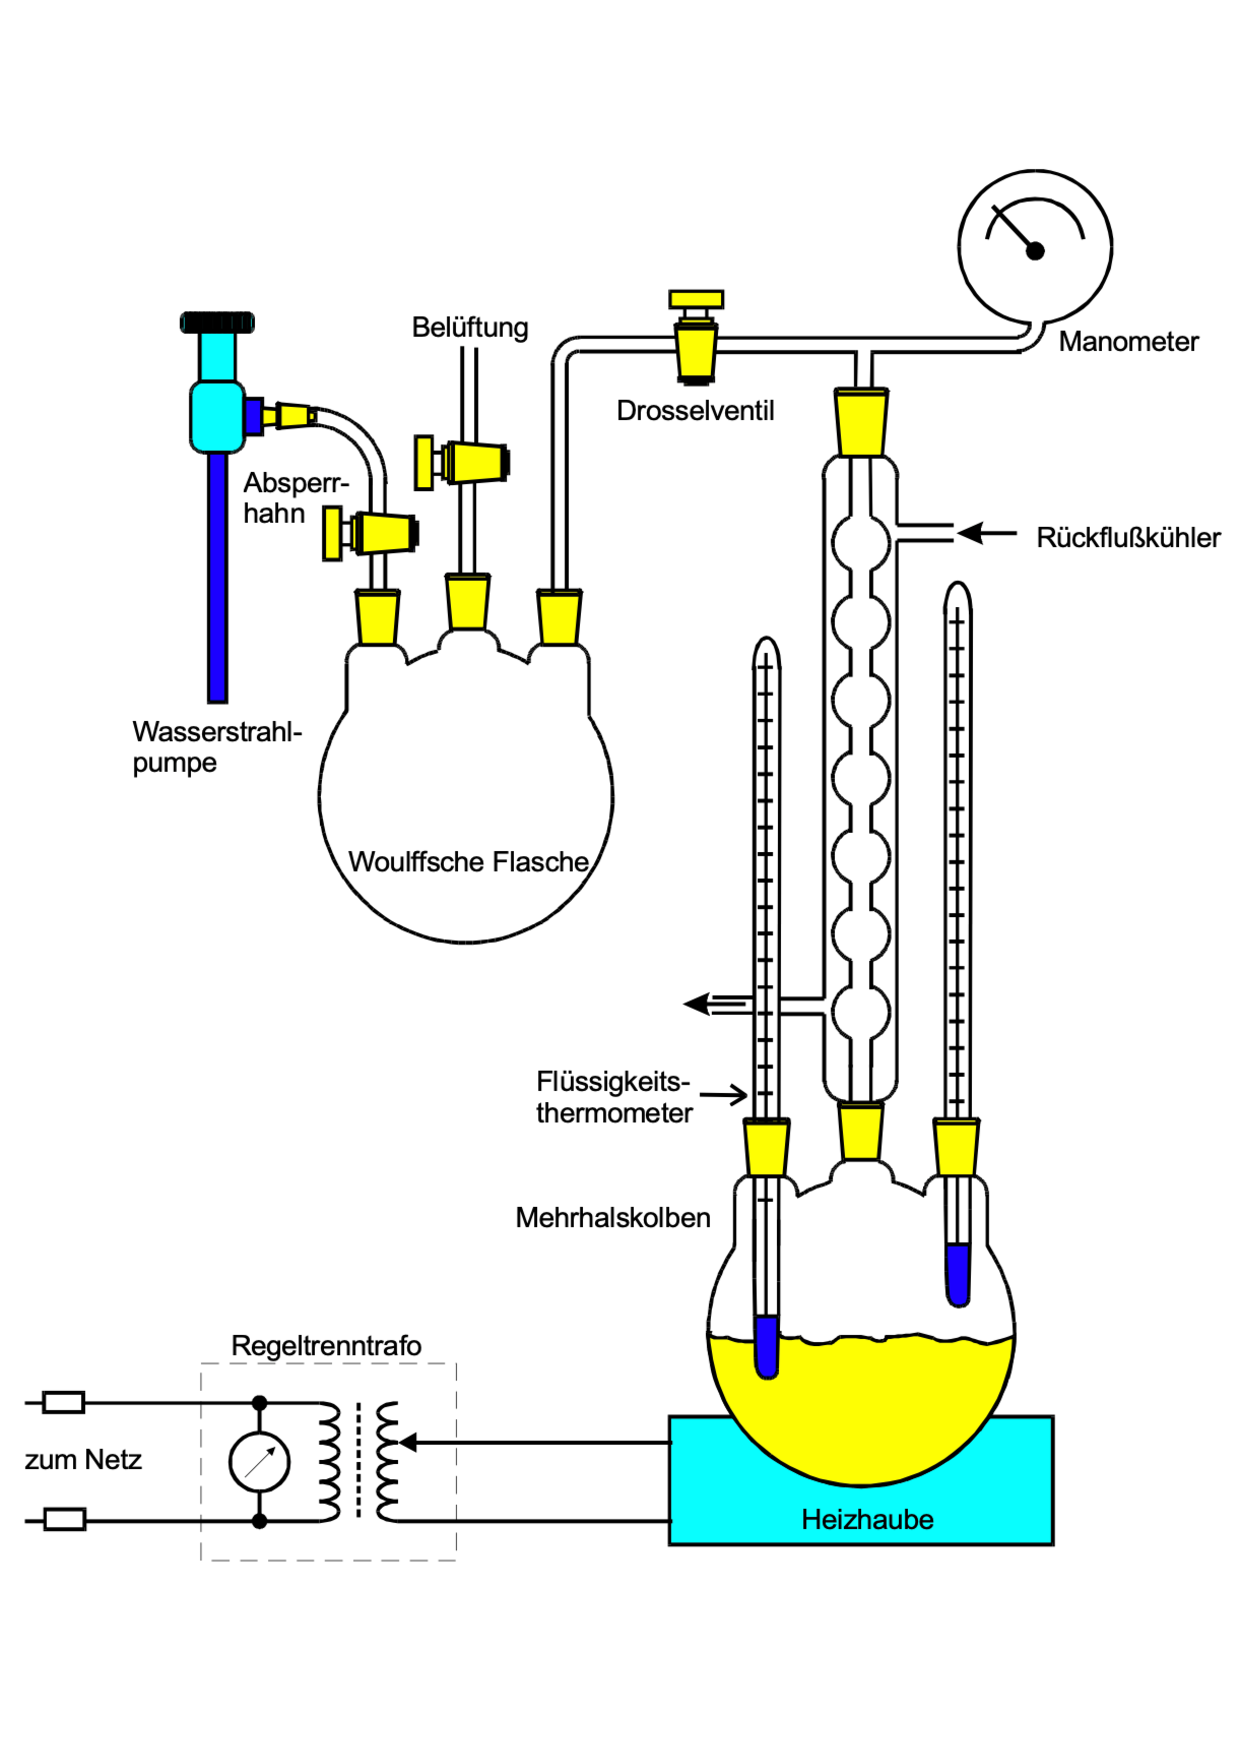
\includegraphics[width=9cm]{aufbau1.pdf}
    \caption{Qualitatives Zustandsdiagramm von Wasser \cite{V203}}
    \label{fig:aufbau1}
  \end{figure}

\noindent
Zuerst wird die Apparatur evakuiert.
Dazu dazu wird das Belüftungsventil geschlossen und der Absperrhahn und das Drosselventil geöffnet. 
Die Wasserstrahlpumpe wird eingeschaltet und läuft bis sich ein konstanter Druck einstellt.
Drosselventil und Absperrhahn werden wieder geschlossen und die Heizhaube eingeschaltet, um das
Wasser im Mehrhalskolben zu erhitzen.
Um den entstehenden Wasserdampf zu kondensieren wird zudem noch die Wasserkühlung eingeschaltet.
Immer wenn sich das Wasser um 5 Grad erhitzt, wird die Temperatur der Luft und der Druck abgelesen.
Die dabei gemessenen Werte befinden sich in Tabelle (\ref{tab:1}). 



\subsection{Messung über 1 bar}
Der Versuchsaufbau ist in Abbildung (\ref{fig:aufbau2}) dargestellt.

\begin{figure}
    \centering
    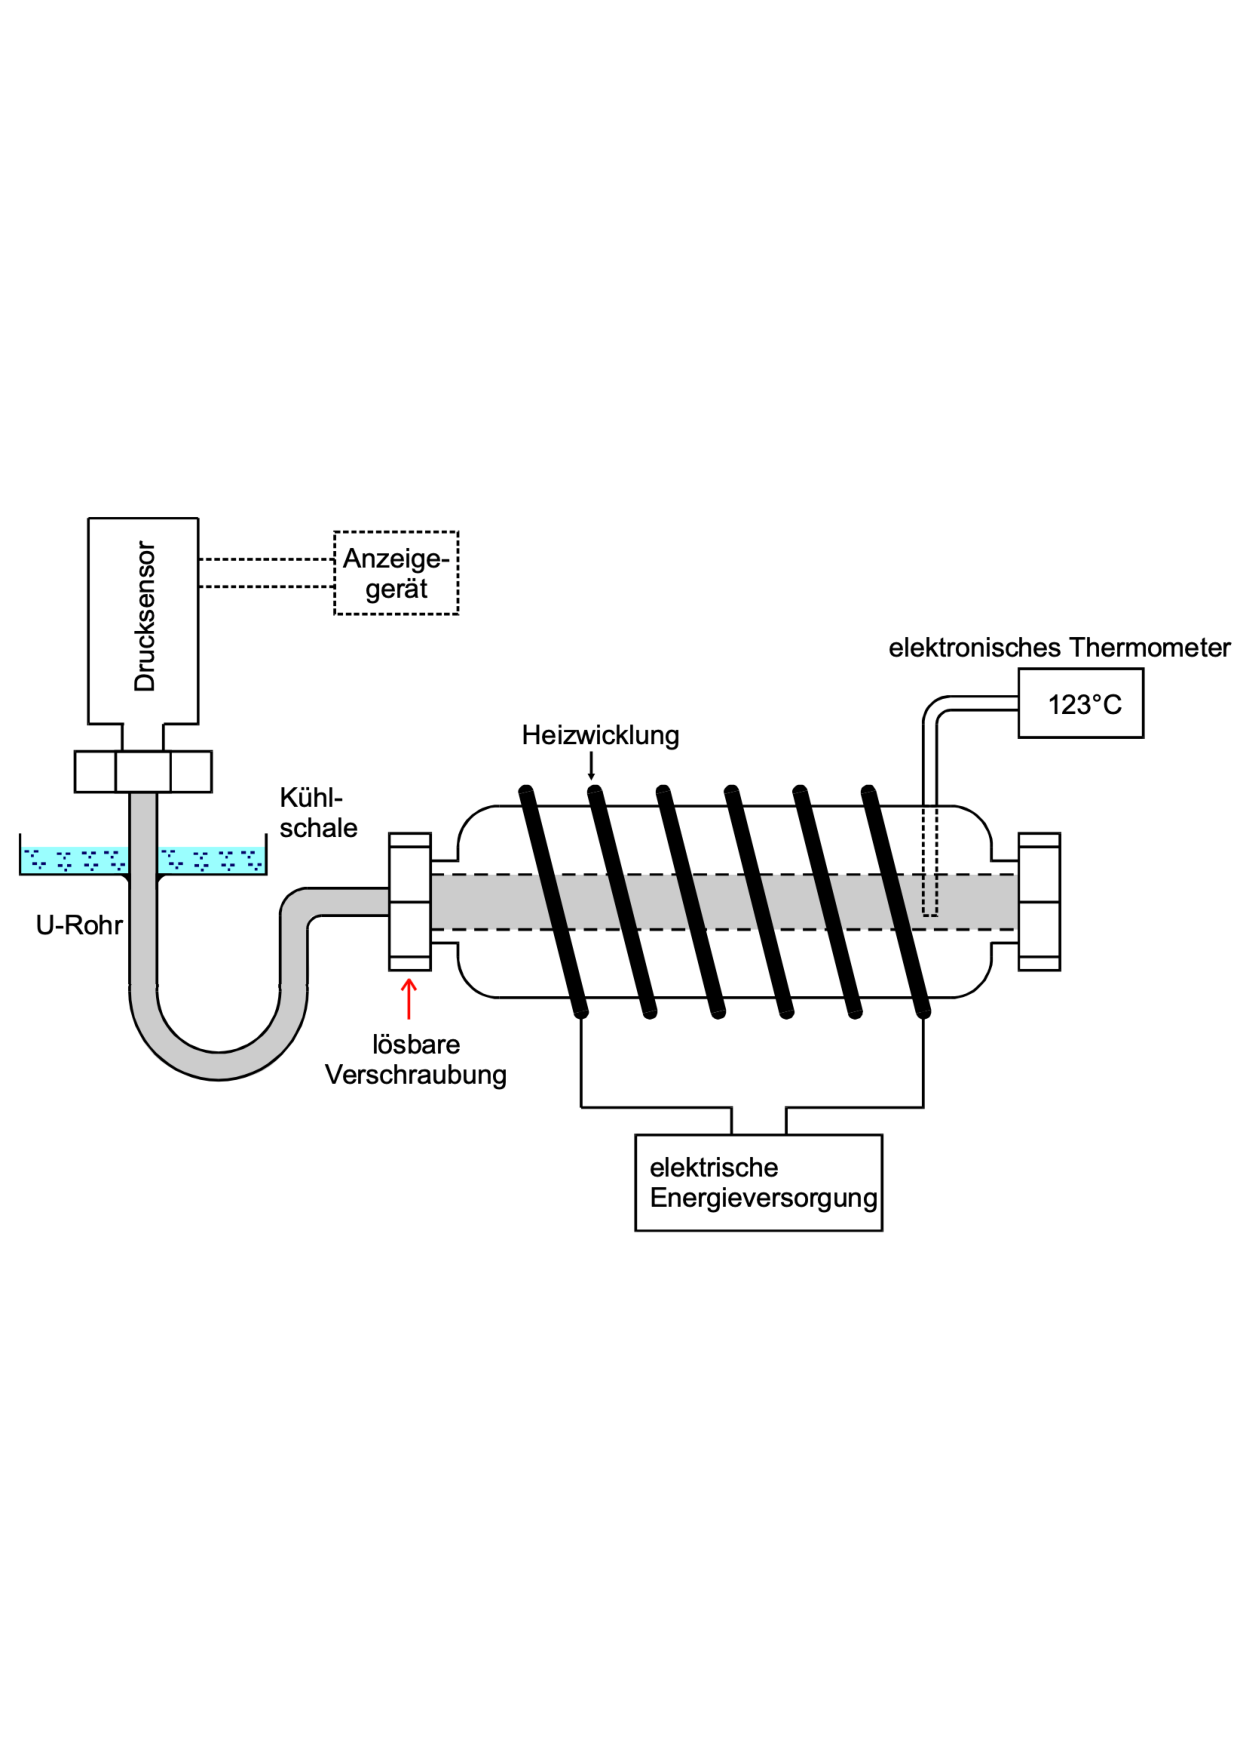
\includegraphics[width=9cm]{aufbau2.pdf}
    \caption{Qualitatives Zustandsdiagramm von Wasser \cite{V203}}
    \label{fig:aufbau2}
  \end{figure}

\noindent
Der Aufbau wird eingeschaltet, sodass der Heizvorgang beginnt.
Sobald der Druck der auf dem Barometer angezeigt wird 1 bar erreicht, 
wird die Temperatur auf dem Thermometer abgelesen.
Dies wird in 1 bar Schritten bis 15 bar wiederholt.
Die dabei gemessenen Werte befinden sich in Tabelle %(\ref{tab:2}).
